\label{sec:pipeline}

In this section the pipeline is presented, which allows to convert an image of an \ac{ECD} into the LTspice schematic file format.
To fully convert the \ac{ECD} from the \ac{IDom} into the \ac{LDom} the following needed conditions have been identified:

\begin{itemize}
    \item the class and position of the \acp{ECC}
    \item the text and position of the annotations as well as the annotation mapping (to which \ac{ECC} belongs this annotation)
    \item the connections between the \acp{ECC}
    \item the conversion into the LTspice schematic file
\end{itemize}

The above points are all embedded into a six-stage pipeline, which can be found in figure \ref{fig:pipeline} and will be thoroughly explained throughout this section.

\begin{figure}
\begin{center}
    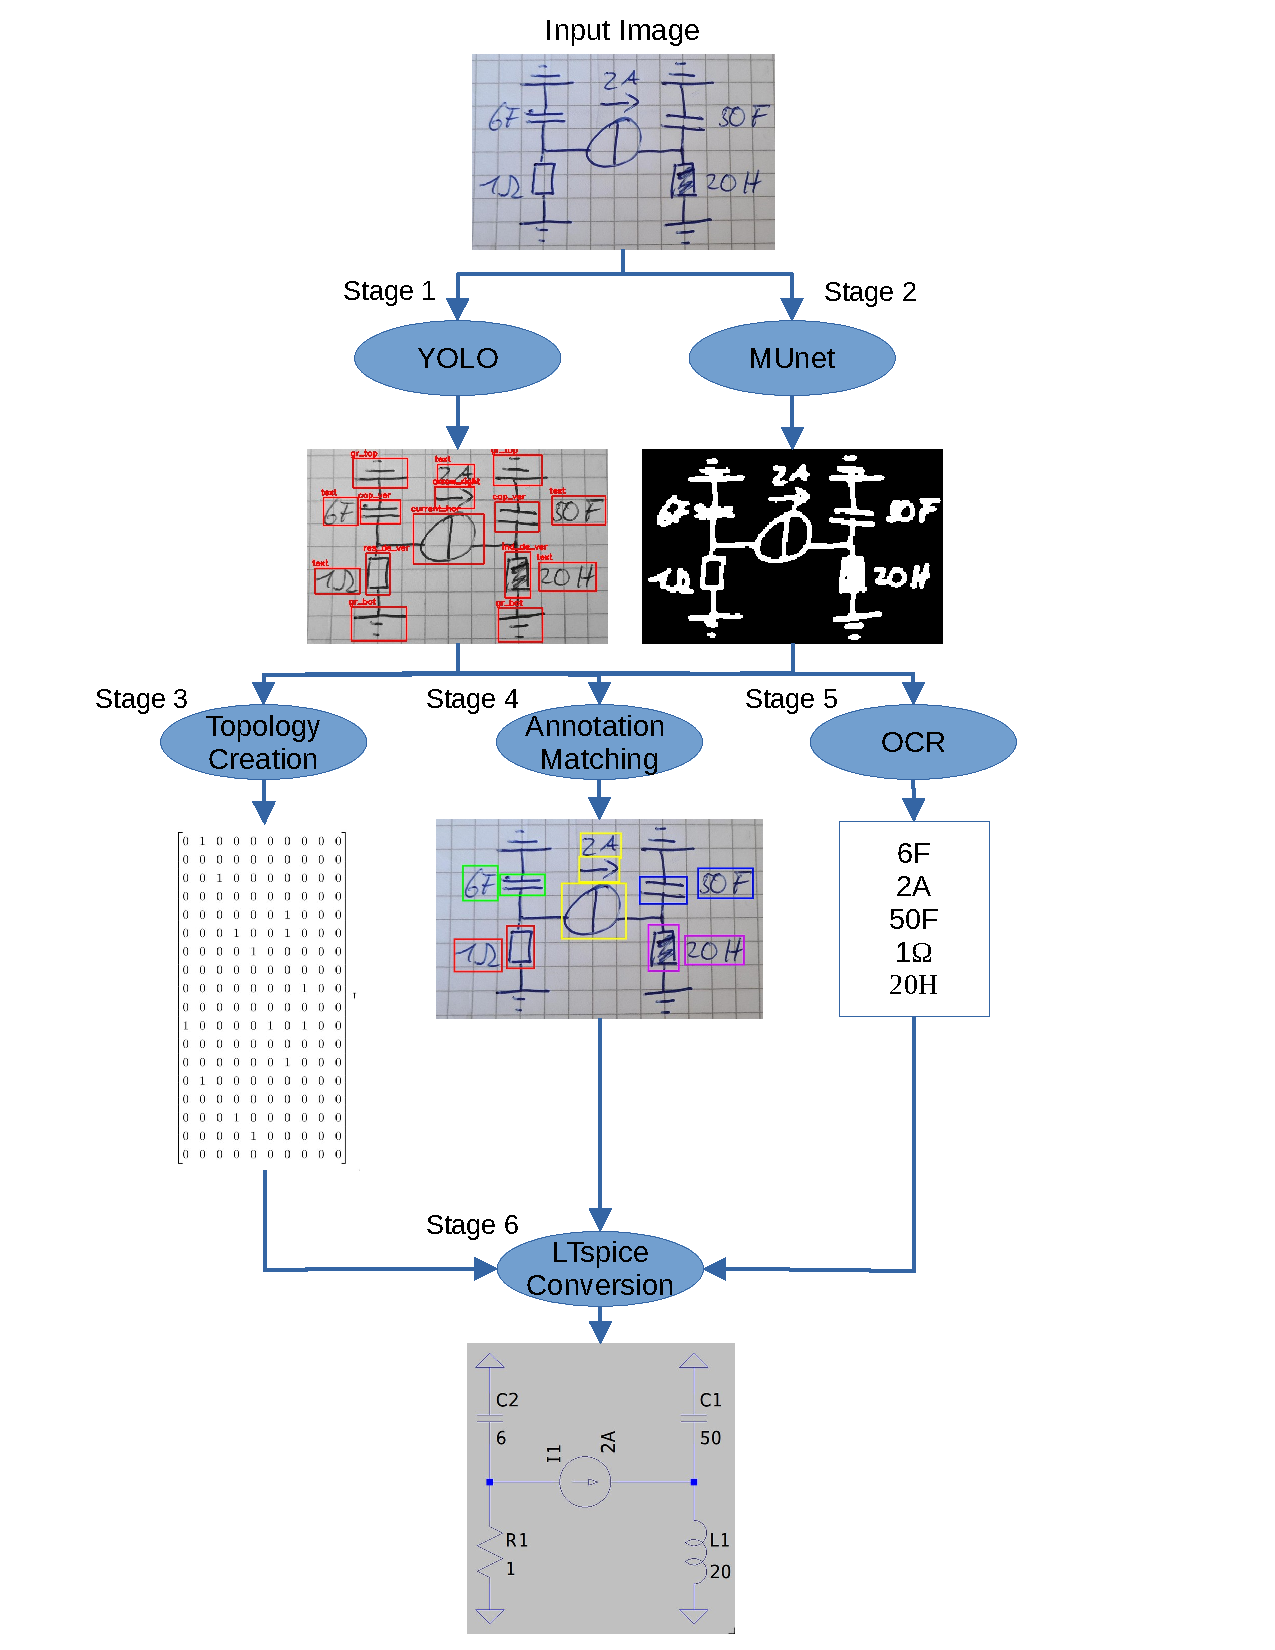
\includegraphics[width=15cm]{imgs/pipeline/pipeline_overview.pdf}
    \caption{The six-stage pipeline presented in this thesis. Stage 1 shows the results of the object detection with \ac{YOLO} and stage 2 the segmentation results with the \ac{MUnet}. Stage 3-5 are postprocessing stages, where the topology is created, the annotations are matched to their respective \ac{ECC} and the characters of the textual annotations are recognized. The last stage is the conversion stage, where the gathered information is embedded into the LTspice schematic file format.}
    \label{fig:pipeline}
\end{center}
\end{figure}


\subsubsection{Stage 1: Object Detection}

Predicting the class and position of an object can essentially be formulated as an object detection problem.
Various object detection networks exist, which could be used for this task.
In this thesis the presented \ac{YOLOv4}-Tiny (section \ref{sec:yolo}), which is from now on referred to as \ac{YOLO}, is used to predict the \acp{ECC}, \ac{ECC}-annotations (arrows for sources) and the text annotations in the \ac{IDom}.
\ac{YOLO} was chosen since it has a good compromise between network size and classification performance.

\subsubsection{Stage 2: Segmentation}

Furthermore, the pipeline includes the segmentation of the circuit.
Segmentation is needed because of the topology building step, which is described next requires a clean mask of the circuit.
The initial clean mask was created using image binarization.
While the topology building worked for circuits with white background it however failed for circuits with checkered background.
Therefore, the \ac{MUnet} (section \ref{sec:mobilenetv2_unet}) is used to segment a circuit in the \ac{IDom}.
The network predicts a binary classification output in the form background / not background, where everything which is unrelated to the \ac{ECD} is considered background.
The network was trained for both checkered and uncheckered backgrounds, such that it can be applied on both types of images.
Again, \ac{MUnet} was chosen, since it is a lightweight network with appropriate performance, able to be used on mobile devices.

% An example prediction of both networks can be seen in figure \ref{fig:example_predictions}.
% \begin{figure}
% \begin{center}
%     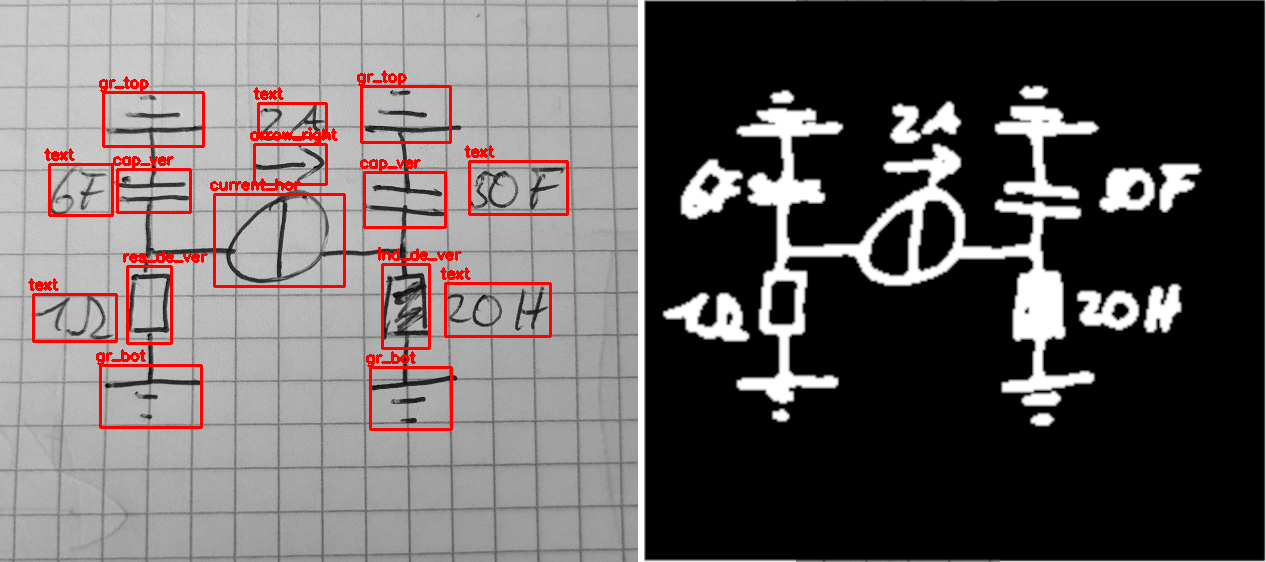
\includegraphics[width=16cm]{imgs/pipeline/combined_pred.png}
%     \caption{Example predictions of YOLO (left) and \ac{MUnet} (right). YOLO predicts a bounding box around each component with its corresponding class, while \ac{MUnet} predicts a segmentation mask a binary fashion of the whole \ac{ECD} drawing, including \ac{ECC} annotations. Primary segmentation is needed to remove the checkered background from the image.}
%     \label{fig:example_predictions}
% \end{center}
% \end{figure}

\subsubsection{Stage 3: Topology Creation}

The next step in the pipeline is the identification of the connections between the \acp{ECC}, such that the wires from the \ac{IDom} can be transformed into the \ac{LDom}.
In an abstract form this is topology creation.
This step does not take into account the spatial positions of the components, but only the semantics of the circuit.
In the following the algorithm is presented, which takes as input the predicted bounding boxes and the segmentation mask of the circuit and produces the topology of the circuit.
The algorithm utilizes various OpenCV algorithms, which are first briefly explained.

\textbf{Connected Components Labeling} by Grana et al. \cite{cca} is an 8-way connectivity algorithm used to label blob like regions in a binary image.
In the topology creation process it is used to identify the wires.

\textbf{Morphological Operations} like erosion, dilation or the combinations of those like opening and closing \cite{cv}, are used to filter the used binary images and to refine results obtained from various sources in the pipeline.

After the basic methods were presented now the algorithm can be explained.
The algorithm receives as input the predicted bounding boxes and the segmentation mask of the circuit.

\begin{enumerate}
    \item Copy the \textbf{SegmentationMask} $\in \{0,1\}^{h \times w}$  into \textbf{WiresOnly}. Iterate over the bounding boxes (bbox $\in \{x_1, y_1, x_2, y_2, class\}$, where $(x_1, y_1)$ represent the upper left corner of the bounding box and $(x_2, y_2)$ the lower right) and remove every pixel in \textbf{WiresOnly}, which is included in a bounding box. Only the wires remain now.
    \item Perform morphological closing on \textbf{WiresOnly} to close up small holes in the wires.
    \item Apply connected components labeling on \textbf{WiresOnly} to label the separate wire blobs resulting in \textbf{WiresLabeled}.
    \item Create a matrix \textbf{BBoxMask} of zeros with the size of \textbf{WiresOnly}. Iterate over the bounding boxes and populate \textbf{BBoxMask} with rectangles with a thin border created from the bounding box coordinates.
    \item Apply the and-operator on \textbf{WiresLabeled} and \textbf{BBoxMask} and receive the intersections, where a wire is intersecting the border of a bounding box. Store the result in \textbf{Intersections}.
    \item Initialize a dictionary \textbf{Topology} and populate it by iterating over \textbf{Intersections} and for each intersection index check the connected components label at this index create an entry in \textbf{Topology} with an empty array.
    \item Iterate over each intersections index and find the bounding box which is ``involved'' in this intersection. A bounding box is ``involved'', when intersection index $\in$ bounding box border and the class of the bounding box is an \ac{ECC}.
    \item Find the orientation of the intersection. Orientation refers to the connection orientation relative to the bounding box, i.e. is the intersection at the top, bottom, left or right border.
    \item Get the connected components label at the intersection index and add a tuple of (bounding box index, orientation) at the respective spot in the \textbf{Topology} if this index with this orientation is not present.
    \item After the initial \textbf{Topology} is build, iterate over it and remove each connected component label, where the involved bounding boxes array has $size = 1$ and the involved bounding box has a contradictory orientation in relation to the predicted class, i.e. classes predicted with vertical orientation can only have a connection at the top or bottom, classes predicted with horizontal orientation can only have a connection left or right.
    \item Return the \textbf{Topology}
\end{enumerate}

\subsubsection{Stage 4: Annotation Matching}

In this thesis different annotations are used.
Arrow annotations are only used for voltage and current sources to indicate the direction of the potential difference as well as the current flow, respectively.
On the other side textual annotations can be applied to any type of an \ac{ECC}.
To fully reflect the circuit in the \ac{LDom} annotations have to be matched against their respective \ac{ECC}.
The algorithm used in this thesis is presented in algorithm \ref{alg:arrow_matching} and \ref{alg:text_matching} for arrow and text annotation respectively.
An annotation is matched against an \ac{ECC} using a simple brute force nearest neighbor approach, based on the center distance of the bounding boxes to match.
Brute force in the sense that every annotation will get matched against an \ac{ECC} without considering that the distance between annotation and \ac{ECC} is maybe way too big, like it would be the case for example when a \ac{FP} annotation is predicted, it certainly will get matched.
Multiple annotations are also possible with this algorithm, but when this occurs the one with the smallest distance is taken and the other match is ignored.

\begin{algorithm}[H]

\SetAlgoLined
\KwIn{\ A = $\{a_1, ..., a_n\}$ (list of predicted arrow  bboxes)

E = $\{e_1, ..., e_o\}$ (list of predicted ECC bboxes)
}
\KwOut{A$_m$ = $\{(a_1, e_i), ..., (a_n, e_j)\}$ (list of arrow bboxes matched against an ECC bbox)}

A$_m$ $\gets$ \{\}\;
\For{a in A} {
    distances $\gets$ \{\}\;
    a$_{center}$ $\gets$ get\_bounding\_box\_center(a)\;

    \For{e in E}{
        \If{is\_source\_type(e)}{
            e$_{center}$ $\gets$ get\_bounding\_box\_center(e)\;
            dist $\gets$ euclidean\_distance(a$_{center}$, e$_{center}$)\;
            distances $\gets$ distances + (dist, a, e)\;
        }
    }

    dist$_{min}$, a$_m$, e$_m$ $\gets$ get\_min\_distance(distances)\;
    A$_m$ $\gets$ A$_m$ + (a$_m$, e$_m$)\;
}

\caption{Arrow Annotation Matching}\label{alg:arrow_matching}
\end{algorithm}

\begin{algorithm}[H]
\caption{Textual Annotation Matching}\label{alg:text_matching}
\SetAlgoLined

\KwIn{T = $\{t_1, ..., t_m\}$ (list of predicted text bboxes)

E = $\{e_1, ..., e_o\}$ (list of predicted ECC bboxes)
}

\KwOut{T$_m$ = $\{(t_1, e_x), ..., (t_m, e_y)\}$ (list of text annotation bboxes matched against an ECC bbox)}

T$_m$ $\gets$ \{\}\;
\For{t in T} {
    distances $\gets$ \{\}\;
    t$_{center}$ $\gets$ get\_bounding\_box\_center(t)\;

    \For{e in E} {
        e$_{center}$ $\gets$ get\_bounding\_box\_center(e)\;
        dist $\gets$ euclidean\_distance(t$_{center}$, e$_{center}$)\;
        distances $\gets$ distances + (dist, t, e)\;
    }

    dist$_{min}$, t$_m$, e$_m$ $\gets$ get\_min\_distance(distances)\;
    T$_m$ $\gets$ T$_m$ + (t$_m$, e$_m$)\;
}

\end{algorithm}


% \begin{bmatrix}
% 	0 & 1 & 0 & 0 & 0 & 0 & 0 & 0 & 0 & 0 &0& 0 & 0 & 0 & 0 & 0 & 0 & 0 & 0 & 0 & 0 & 0 & 1 & 0 & 0 & 0 & 0 & 0 & 0 & 0\\
%     0 & 0 & 0 & 0 & 0 & 0 & 0 & 0 & 0 & 0 &0& 0 & 0 & 0 & 0 & 0 & 1 & 0 & 0 & 0 & 0 & 0 & 0 & 1 & 0 & 0 & 1 & 0 & 0 & 0\\
%     0 & 0 & 0 & 0 & 1 & 0 & 0 & 0 & 0 & 0 &0& 0 & 0 & 0 & 0 & 0 & 0 & 0 & 0 & 0 & 0 & 0 & 0 & 0 & 0 & 0 & 0 & 1 & 0 & 0\\
%     0 & 0 & 0 & 0 & 0 & 0 & 0 & 0 & 0 & 0 &1& 0 & 0 & 0 & 0 & 1 & 0 & 1 & 0 & 0 & 0 & 0 & 0 & 0 & 0 & 0 & 0 & 0 & 0 & 0\\
%     0 & 0 & 0 & 0 & 0 & 0 & 1 & 0 & 0 & 0 &0& 1 & 0 & 0 & 0 & 0 & 0 & 0 & 0 & 0 & 0 & 0 & 0 & 0 & 0 & 0 & 0 & 0 & 0 & 0\\
%     0 & 0 & 0 & 1 & 0 & 0 & 0 & 0 & 0 & 0 &0& 0 & 0 & 0 & 1 & 0 & 0 & 0 & 0 & 0 & 0 & 0 & 0 & 0 & 0 & 0 & 0 & 0 & 0 & 0\\
% \end{bmatrix}

\subsubsection{Stage 5: Optical Character Recognition of Textual Annotations}

Interpretation of the textual annotations should normally be also part of the pipeline.
Due to time constraints this step was not implemented in the scope of this thesis.
But an \ac{OCR} engine such as Tesseract \cite{tesseract}, could be used to detect the characters in the textual annotations.

\subsubsection{Stage 6: LTspice Conversion}

The last step in the proposed pipeline is the embedding of the gathered information into the LTspice schematic file, where the syntax was presented in section \ref{sec:ltspice}.
A module was created, which utilizes this syntax and generates a LTspice schematic file, where \acp{ECC} can be directly parametrized with their properties by passing the respective values to the generator functions.
Three input values can be found for the generator functions:
\begin{itemize}
    \item \ac{ECC} type
    \item annotation parameters (no input provided in this work)
    \item position of the \ac{ECC}
\end{itemize}

Further the module can also generate wires to connect the \acp{ECC}, here only the start and end position of the wire have to be passed to the generator functions.

So far, the impact of the position of an \ac{ECC} was not discussed, but to replicate the circuit in the \ac{LDom} it is necessary to capture the positions in the \ac{IDom}.
Positions from the \ac{IDom} were predicted by the \ac{YOLO} network and are available as a bounding box, containing class, size and the center point of an \ac{ECC}.

It was mentioned that LTspice relies on a $32 \times 32$ grid, where \acp{ECC} and wires are aligned to.
\acp{ECC} from the \ac{IDom} need to be projected into that grid.
A simple approach would be to take the minimum distance between two \acp{ECC} in the \ac{IDom} and use this distance as a grid normalizer.
The problem is here that, the sizes and aspect ratios of bounding boxes do not correspond to the sizes in the \ac{LDom}.
So when just using the minimum distance it can happen, that two \ac{ECC} components will overlap.
To mitigate this issue an additional $stretch \in \R^+$ parameter is introduced, which scales the minimum distance.
A $stretch < 1$ will reduce the minimum distance between the \acp{ECC} in the \ac{IDom} and increase the distance in the \ac{LDom}.
The coordinates in the \ac{LDom} can then be calculated with:

\begin{equation}
    coord_{LDom} = \text{round}\left(\frac{coord_{IDom}}{stretch \cdot dist_{min}}\right) \cdot 32
    \label{eq:ldom_pos}
\end{equation}

Where, $coord_*$ corresponds to the x and y coordinate respectively.
A stretch of $0.3$ has shown to provide a good balance between enough space between components for them to not intersect and at the same time not overscaling the distances between the \acp{ECC} too much.
